\documentclass[11pt]{article}

\usepackage{times}
\usepackage{epsf}
\usepackage{epsfig}
\usepackage{amsmath, alltt, amssymb, xspace}
\usepackage{wrapfig}
\usepackage{fancyhdr}
\usepackage{url}
\usepackage{verbatim}
\usepackage{fancyvrb}

\usepackage{subfigure}
\usepackage{cite}
\usepackage{hyperref}
\hypersetup{%
    pdfborder = {0 0 0}
}
%\usepackage{cases}
%\usepackage{ltexpprt}
%\usepackage{verbatim}

%\topmargin      -0.70in  % distance to headers
%\headheight     0.2in   % height of header box
%\headsep        0.4in   % distance to top line
%\footskip       0.3in   % distance from bottom line

% Horizontal alignment
\topmargin      -0.50in  % distance to headers
\oddsidemargin  0.0in
\evensidemargin 0.0in
\textwidth      6.5in
\textheight     8.9in 


%\centerfigcaptionstrue

%\def\baselinestretch{0.95}


\newcommand\discuss[1]{\{\textbf{Discuss:} \textit{#1}\}}
%\newcommand\todo[1]{\vspace{0.1in}\{\textbf{Todo:} \textit{#1}\}\vspace{0.1in}}
\newtheorem{problem}{Problem}[section]
%\newtheorem{theorem}{Theorem}
%\newtheorem{fact}{Fact}
\newtheorem{define}{Definition}[section]
%\newtheorem{analysis}{Analysis}
\newcommand\vspacenoindent{\vspace{0.1in} \noindent}

%\newenvironment{proof}{\noindent {\bf Proof}.}{\hspace*{\fill}~\mbox{\rule[0pt]{1.3ex}{1.3ex}}}
%\newcommand\todo[1]{\vspace{0.1in}\{\textbf{Todo:} \textit{#1}\}\vspace{0.1in}}

%\newcommand\reducespace{\vspace{-0.1in}}
% reduce the space between lines
%\def\baselinestretch{0.95}

\newcommand{\fixmefn}[1]{ \footnote{\sf\ \ \fbox{FIXME} #1} }
\newcommand{\todo}[1]{
\vspace{0.1in}
\fbox{\parbox{6in}{TODO: #1}}
\vspace{0.1in}
}

\newcommand{\mybox}[1]{
\vspace{0.2in}
\noindent
\fbox{\parbox{6.5in}{#1}}
\vspace{0.1in}
}


\newcounter{question}
\setcounter{question}{1}

\newcommand{\myquestion} {{\vspace{0.1in} \noindent \bf Question \arabic{question}:} \addtocounter{question}{1} \,}

\newcommand{\myproblem} {{\noindent \bf Problem \arabic{question}:} \addtocounter{question}{1} \,}



\newcommand{\copyrightnotice}[1]{
\vspace{0.1in}
\fbox{\parbox{6in}{\small Copyright \copyright\ 2014\ \ Wenliang Du, Syracuse University.\\
      The development of this document is/was funded by the following grants from
      the US National Science Foundation: No. 1303306 and 1318814.
      This lab was altered and imported into the Labtainer framework by the Naval Postgraduate
      School, Center for Cybersecurity and Cyber Operations under National Science
      Foundation Award No. 1438893.
      Permission is granted to copy, distribute and/or modify this document
      under the terms of the GNU Free Documentation License, Version 1.2
      or any later version published by the Free Software Foundation.
      A copy of the license can be found at http://www.gnu.org/licenses/fdl.html.}}
\vspace{0.1in}
}

\newcommand{\copyrightnoticeA}[1]{
\vspace{0.1in}
\fbox{\parbox{6in}{\small Copyright \copyright\ 2006\ \ Wenliang Du, Syracuse University.\\
      The development of this document was partially funded by
      the National Science Foundation's Course, Curriculum, and Laboratory
      Improvement (CCLI) program under Award No. 0618680 and 0231122.
      This lab was altered and imported into the Labtainer framework by the Naval Postgraduate
      School, Center for Cybersecurity and Cyber Operations under National Science
      Foundation Aware No. 1438893.

      Permission is granted to copy, distribute and/or modify this document
      under the terms of the GNU Free Documentation License, Version 1.2
      or any later version published by the Free Software Foundation.
      A copy of the license can be found at http://www.gnu.org/licenses/fdl.html.}}
\vspace{0.1in}
}


\newcommand{\nocopyrightnotice}[1]{
\vspace{0.1in}
\fbox{\parbox{6in}{\small  
      The development of this document is funded by 
      the National Science Foundation's Course, Curriculum, and Laboratory 
      Improvement (CCLI) program under Award No. 0618680 and 0231122. 
      Permission is granted to copy, distribute and/or modify this document.
      }}
\vspace{0.1in}
}

\newcommand{\idea}[1]{
\vspace{0.1in}
{\sf IDEA:\ \ \fbox{\parbox{5in}{#1}}}
\vspace{0.1in}
}

\newcommand{\questionblock}[1]{
\vspace{0.1in}
\fbox{\parbox{6in}{#1}}
\vspace{0.1in}
}


\newcommand{\minix}{{\tt Minix}\xspace}
\newcommand{\unix}{{\tt Unix}\xspace}
\newcommand{\linux}{{\tt Linux}\xspace}
\newcommand{\ubuntu}{{\tt Ubuntu}\xspace}
\newcommand{\selinux}{{\tt SELinux}\xspace}
\newcommand{\freebsd}{{\tt FreeBSD}\xspace}
\newcommand{\solaris}{{\tt Solaris}\xspace}
\newcommand{\windowsnt}{{\tt Windows NT}\xspace}
\newcommand{\setuid}{{\tt Set-UID}\xspace}
%\newcommand{\smx}{{\tt Smx}\xspace}
\newcommand{\smx}{{\tt Minix}\xspace}
\newcommand{\relay}{{\tt relay}\xspace}
\newcommand{\isys}{{\tt iSYS}\xspace}
\newcommand{\ilan}{{\tt iLAN}\xspace}
\newcommand{\iSYS}{{\tt iSYS}\xspace}
\newcommand{\iLAN}{{\tt iLAN}\xspace}
\newcommand{\iLANs}{{\tt iLAN}s\xspace}
\newcommand{\bochs}{{\tt Bochs}\xspace}

\newcommand\FF{{\mathcal{F}}}

\newcommand{\argmax}[1]{
\begin{minipage}[t]{1.25cm}\parskip-1ex\begin{center}
argmax
#1
\end{center}\end{minipage}
\;
}

\newcommand{\bm}{\boldmath}
\newcommand  {\bx}    {\mbox{\boldmath $x$}}
\newcommand  {\by}    {\mbox{\boldmath $y$}}
\newcommand  {\br}    {\mbox{\boldmath $r$}}


%\pagestyle{fancyplain}
%\lhead[\thepage]{\thesection}      % Note the different brackets!
%\rhead[\thesection]{SEED Laboratories}
%\lfoot[\fancyplain{}{}]{Syracuse University} 
%\cfoot[\fancyplain{}{}]{\thepage} 

\newcommand{\tstamp}{\today}   
%\lhead[\fancyplain{}{\thepage}]         {\fancyplain{}{\rightmark}}
%\chead[\fancyplain{}{}]                 {\fancyplain{}{}}
%\rhead[\fancyplain{}{\rightmark}]       {\fancyplain{}{\thepage}}
%\lfoot[\fancyplain{}{}]                 {\fancyplain{\tstamp}{\tstamp}}
%\cfoot[\fancyplain{\thepage}{}]         {\fancyplain{\thepage}{}}
%\rfoot[\fancyplain{\tstamp} {\tstamp}]  {\fancyplain{}{}}

\pagestyle{fancy}
%\lhead{\bfseries Computer Security Course Project}
\lhead{\bfseries SEED Labs}
\chead{}
\rhead{\small \thepage}
\lfoot{}
\cfoot{}
\rfoot{}




\begin{document}

\begin{center}
{\LARGE IPTables for Industrial Control Systems (iptables-ics)}
\vspace{0.1in}\\
\end{center}


\section{Overview}
This Labtainer exercise illustrates the use of iptables
to limit network access to a PLC component in an operational
technology (OT) environment. This control is provided by 
a component serving as a firewall, as illustrated in Figure 
\ref{fig:topology}.

When properly configured, the firewall will only allow the following traffic
between the clients and the PLC:
\begin{itemize}
\item Client 1 can only access the PLC via SSH and HTTP (port 8080).
\item Client 2 can only access the PLC via MODBUS TCP and HTTP (ports 80 and 8080).
\end{itemize}

\subsection {Background}
Industrial control systems often use IP based networks to communicate with
other components.  Just as is the case with many information technology (IT) networks,
protection of assets may depend on limiting the types of network traffic 
permitted to flow between components.  For example, web traffic (e.g., HTTP)
might only be permitted to enter a given component if it originates from specific
sources.

A variety of different techniques and products exist for the purpose of limiting
IP traffic in IT and OT systems.  In this lab, you will limit IP traffic through
use of Linux iptables.  
The student is expected to have separately learned about the use of iptables
to selectively block network traffic. The firewall component includes a few
example firewall setting scripts that you can reference.  The manpage for iptables can be viewed on the
firewall component using:
\begin{verbatim}
   man iptables
\end{verbatim}

Students are expected to have a basic 
familiarity with the Linux command line, and the ability to edit files and
run simple shell scripts. Some experience with Wireshark is presumed, e.g., performance of
the wireshark-intro lab.

\section{Lab Environment}
This lab runs in the Labtainer framework,
available at http://my.nps.edu/web/c3o/labtainers.
That site includes links to a pre-built virtual machine
that has Labtainers installed, however Labtainers can
be run on any Linux host that supports Docker containers.

From your labtainer-student directory start the lab using:
\begin{verbatim}
    labtainer iptables-ics
\end{verbatim}
\noindent A link to this lab manual will be displayed.  


\begin{figure}[H]
\begin{center}
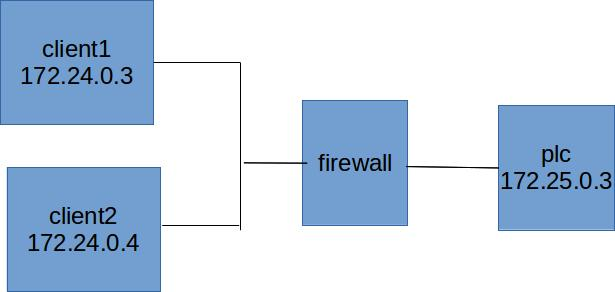
\includegraphics [width=0.8\textwidth]{iptables-ics.jpg}
\end{center}
\caption{Network topology for the iptables-ics lab}
\label{fig:topology}
\end{figure}

\section{Lab Tasks}
\subsection{Explore}
The Wireshark utility is installed on the firewall. 
Use it to view network traffic through the firewall, and to 
debug your firewall rules.  Start it from the firewall terminal:
\begin{verbatim}
wireshark &
\end{verbatim}
\noindent Then select the eth0 interface.

On both the client1 and client2 terminals use the following applications
to explore the services offered by PLC:

\begin{verbatim}
        ./mbtcp-simple.py
\end{verbatim}
This starts a simple MODBUS client.  Observe the network traffic using
wireshark, making note of the destination TCP port number used by the client when
connecting to the PLC. Then use {\tt <ctrl C>} to terminate the program on each client.

\noindent Start firefox on each client:
\begin{verbatim}
        firefox &
\end{verbatim}
\noindent and point the browswer to the following two URLs:
\begin{verbatim}
        http://plc:8080
        http://plc
\end{verbatim}
\noindent Observe the traffic in wireshark, making note the
source IP addresses and the destination ports used by the 
clients when connecting to the PLC.

\noindent Finally, use SSH to connect to the PLC from each client:
\begin{verbatim}
        ssh plc
\end{verbatim}
\noindent There is no need to login.  After observing the initial traffic,
use {\tt <ctrl C>} to exit from ssh.

\subsection{Use iptables to limit traffic}
The iptables utility is installed on the ``firewall'' component.
Use it to prevent the firewall from forwarding any traffic
to the PLC other than specified below.

\begin{enumerate}
\item Client 1 can only access the PLC via SSH and HTTP 
(with port 8080 only).
\item Client 2 can only access the PLC via MODBUS TCP and HTTP 
(with ports 8080 and 80).
\item No other network traffic is permitted to reach the PLC
\end{enumerate}

You may reference and experiment with the example firewall scripts that
are on the firewall component in the home directory.  \textbf{NOTE:} The IP addresses in the example
script may not correspond to the IP addresses of your system, and would
therefore need to be changed.  To run the {\tt example\_fw.sh} script, use:
\begin{verbatim}
        sudo ./example_fw.sh
\end{verbatim}
View the content of the scripts to understand what they do.
Consider putting your iptables commands in a script so it is easy
to test and reconfigure the iptables if you restart the lab.
Note that the last line of {\tt example\_fw.sh} directs iptables
to send log messages to a file that is at:
\begin{verbatim}
  /var/log/iptables.log
\end{verbatim}
\noindent If you include that directive in your configuration, you can observe when
iptables drops filtered packets, e.g., by tailing the log from one of the 
firewall terminal tabs:
\begin{verbatim}
  tail -f /var/log/iptables.log
\end{verbatim}

After configuring iptables to meet the requirements, use the applications on Client1 and Client2 to
demonstrate that the firewall only allows the desired traffic.
Watch the traffic in wireshark to confirm the TCP handshake fails
when attempting to connect to filtered ports.  

When you believe you have the proper iptables configuration and have tested it,
use the {\tt stoplab} command from your Linux system.  You are free to then restart
the lab using {\tt labtainer iptables-ics} and explore further without concern for
the state of the system when you again stop it.  Alternately, if the {\tt checkwork} command is
available on your distribution, you can use that command from the Linux system instead of {\tt stoplab}, and then just
continue working.

\section{Submission}
After finishing the lab, go to the terminal on your Linux system that was used to start the lab and type:
\begin{verbatim}
    stoplab 
\end{verbatim}
When you stop the lab, the system will display a path to the zipped lab results on your Linux system.  Provide that file to 
your instructor, e.g., via the Sakai site.

\copyrightnotice

\end{document}
